\documentclass{report}
\title{Appendix 4}
\date{Started 15 April 2025}
\author{Malcolm}
\usepackage{amsmath} %import math
\usepackage{mathtools} %more math
\usepackage{amssymb} %for QED symbol
\usepackage{amsthm} %
\usepackage{bm}%bold math
\usepackage{graphicx} %import imaging
\graphicspath{{./images/}} %set imaging path
\begin{document}
\maketitle

\tableofcontents

\newpage
\section{Real Numbers}
\subsection{Dedekind Cuts}
\textbf{Motivation}\\
Recall the definitions:
\begin{itemize}
\item The set $\mathbb{N}$ of natural numbers, 1, 2, 3, 4,\ldots
\item The set $\mathbb{Z}$ of integers, 0, 1, -1, -2, 2,\ldots 
\item The set $\mathbb{Q}$ of rational numbers $p/q$ where $p,q$ are integers, $q\neq0$.
\end{itemize}
It is clear that $\mathbb{N}\subset\mathbb{Z}\subset\mathbb{Q}$. Intuitively $\mathbb{Z}$ improves $\mathbb{N}$ 
because it contains negatives and $\mathbb{Q}$ improves $\mathbb{Z}$ because it contains reciprocals. However
notice that $\mathbb{Q}$ is incomplete---doesn't admit irrational roots such as $\sqrt{2}$ or numbers like $\pi$. 
We solve this with $\mathbb{R}$ such that
\begin{equation*}
\mathbb{N}\subset\mathbb{Z}\subset\mathbb{Q}\subset\mathbb{R}
\end{equation*}
As an example of the fact that $\mathbb{Q}$ is incomplete:\\
\vspace{1mm}\\
\textbf{Theorem} \textit{No number $r$ in $\mathbb{Q}$ has the square equal to 2; that is, 
$\sqrt{2}\notin\mathbb{Q}$.}\\
\vspace{1mm}\\
\textbf{Proof} To prove that every $r=p/q$ has $r^2\neq2$ we show that $p^2\neq2q^2$. (since $r=p/q\neq2\implies
r^2=p^2/q^2\neq2$) We also assume that $p$ and $q$ have no common factors since they would
have been canceled out beforehand.\\
\vspace{1mm}\\
\underline{Case 1}: $p$ is odd. Then $p^2$ is odd while $2q^2$ is not. Therefore $p^2\neq2q^2$.\\
\vspace{1mm}\\
(an even number $n$ would also have even $n^2$: because $n=2a$ for some $a$ would have a square $n^2=4a^2$ 
which is also divisible by 2. An odd number squared is odd: the expression $(n+1)$ for even $n$ 
is odd; its square $(n+1)^2=n^2+2n+1$ is also odd, since $n^2+2n$ is even.)\\
\vspace{1mm}\\
\underline{Case 2}: $p$ is even. Since $p$ and $q$ have no common factors, $q$ is odd. Then $p^2$ is divisible by 4
while $2q^2$ is not (since $q^2$ is odd). Therefore
$p^2\neq2q^2$.\\
\vspace{1mm}\\
Since $p^2\neq2q^2$ for all integers $p$, there is no rational number $r=p/q$ whose square is 2.\qed\\
(next page)\newpage
\noindent\textbf{Dedekind cuts}\\
The set $\mathbb{Q}$ of rational numbers is incomplete with `gaps' of negligible width. An elegant method
to fill in these gaps are with \textit{Dedekind cuts} in which one visualises real numbers as places on a number
line that can be `cut':
\begin{center}
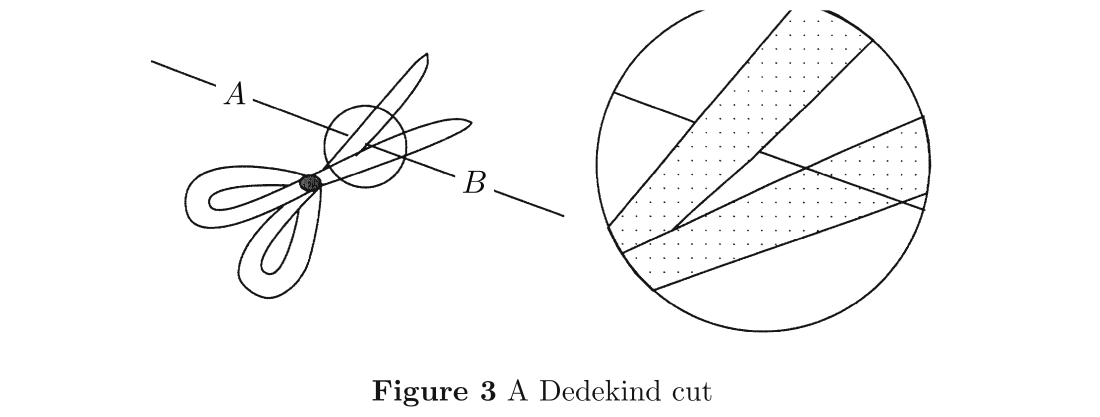
\includegraphics[width=10cm]{1}\\
\end{center}
\textbf{Definition} A \textit{cut} in $\mathbb{Q}$ is a pair of subsets $A,B$ of $\mathbb{Q}$ such that
\begin{itemize}
\item $A\cup B=\mathbb{Q},\,A\neq\emptyset,\,B\neq\emptyset,\,A\cap B=\emptyset$
\item If $a\in A$ and $b\in B$ then $a<b$
\item $A$ contains no largest element
\end{itemize}
$A$ is the left-hand part of the cut and $B$ the right. We denote the cut as $x=A|B$. Now we define:\\
\vspace{1mm}\\
\textbf{Definition} A \textit{real number} is a cut in $\mathbb{Q}$\\
\vspace{1mm}\\
$\mathbb{R}$ is the class (of set-pairs) of all real numbers $x=A|B$. Here are two examples of cuts:
\begin{enumerate}
\item $A|B=\{r\in\mathbb{Q}:r<1\}|\{r\in\mathbb{Q}:r\geq1\}$
\item $A|B=\{r\in\mathbb{Q}:r\leq0$ or $r^2<2\}|\{r\in\mathbb{Q}:r>0$ and $r^2\geq2\}$
\end{enumerate}
The first cut is a \textit{rational cut}, where for some fixed rational number $c$, $A$ is the set of all rationals
$<c$ while $B$ is the rest of $\mathbb{Q}$. We write $c^*$ for the rational cut at $c$.










\end{document}
